\documentclass{article}

%\usepackage{tabularx} 
\usepackage{pdflscape} % For producing landscape pages in PDF documents
\usepackage{afterpage} % For page specific formatting
\usepackage{capt-of}
\usepackage{booktabs} % For controlling the style of tables (specifically the lines)
\usepackage{geometry} % For controlling the positioning of tables
\usepackage{listings} % For adding code snippets to document
\usepackage{parskip} % For making the paragraphs not indent
\usepackage{textcomp} % For making tilde characters that look nice
\usepackage{enumitem} % For controlling the indentation of enumerate lists
\usepackage{changepage} % This allows for temporary indenting of paragraphs
\usepackage{color} % Allows for the definition of colors
\usepackage{graphicx}% Include figure files

% This sets some variables to control the indentation and spacing between paragraphs
\newlength\tindent
\setlength{\tindent}{\parindent}
\setlength{\parindent}{0pt}
\renewcommand{\indent}{\hspace*{\tindent}}

% This defines some colors for displaying syntax highlighting of code
\definecolor{dark-green}{rgb}{0,0.5,0}
\definecolor{purple}{rgb}{0.4,0,0.7}
\definecolor{dark-blue}{rgb}{0.2,0,0.5}
\definecolor{black}{rgb}{0,0,0}

% This sets up the code display function
\lstset{	language=Python,
		basicstyle=\footnotesize,
        	showstringspaces=false,
        	keywordstyle=\color{dark-blue}\ttfamily,
        	stringstyle=\color{purple}\ttfamily,
        	commentstyle=\color{dark-green}\ttfamily,
		identifierstyle=\color{black}\ttfamily,
        	breaklines=true
       }

\begin{document}

\title{PIV Code Development Guidelines}
\date{\today}
\author{Roderick R. La Foy}
\maketitle

\section{\label{sec:level1}Introduction}

This document is designed to be a general purpose reference resource for the development of experimental fluid dynamics research software.  Specifically this document primarily discusses the conventions and standards that should be used for PIV/PTV development.

\section{\label{sec:level1}PIV Code Project Management}

This section primarily discusses the previous versions of the PIV code, the project management, and the over-arching project goals.  The items discussed in this section are good to keep in mind while proceeding on any coding project, but are particularly relevant to the development of the new PIV code. 

\subsection{\label{sec:level1}Previous PIV Code Versions}

There are two previous versions of PIV code that may be referenced for the development of the new PIV code.  These two pieces of software were written under very different conditions and should be used differently while developing new code.

The first version of the code is known as `Prana' and was developed from roughly 2008 to 2014.  This code has been validated extensively and is known to work very well under a wide array of conditions, so this code is useful for validating the velocity field output of the new code.  Additionally the algorithms in the `Prana' code have been exhaustively tested, so the code should also be used as a reference for PIV algorithms that properly account for edge cases and other exceptional programming cases. However the `Prana' code was written without any clear set of guidelines or goals and was written in a piecemeal fashion over several years, so the code is very difficult to read.  Thus this code should not be used as a reference for stylistic purposes or as an example of properly designed code.  In general, referencing `Prana' may be difficult due to the poor readability of the code.

The second version of the code is known as `piv\_3d\_10' and was developed during 2014 for the 4\textsuperscript{th} International PIV Challenge.  This code has been validated in only a small number of situations and additionally has only been used for processing a small number of data sets.  However the `piv\_3d\_10' is extensively well commented, uses appropriate naming conventions, and is organized in a highly algorithmic manner.  Thus this code is very useful for referencing when writing new code, but the code should be used less extensively for testing the output velocity field data.  The `piv\_3d\_10' code may be considered to be an example of well designed code.

Although a large amount of time was put into developing both of these two pieces of software, it is still possible that bugs may exist in the codes.  Thus it is highly recommended that the developers of the new PIV code reference any relevant papers, textbooks, et cetera while writing new algorithms.  Additionally validating new codes against commercial software such as the LaVision DaVis software may be useful as well.

The new version of the PIV code should be considered to be a new version of `Prana' and will be referenced using this convention for the remainder of this document.

\subsection{\label{sec:level1}Management}

A large scale project needs someone (or a small number of people) to coherently manage the project from start to finish.  The person or people performing this task may change over time, but without clearly defined project goals and structuring, the project will become disorganized and may not be completed.  The people performing this task will be in charge of breaking up the project into individual tasks that can be assigned to the various developers on the project.  The managers will then be responsible for ensuring that the individual codes can be combined together into the full project.  Additionally the managers must ensure that all the code that is submitted is readable, well documented, and correctly accomplishes the goal that the code was intended to accomplish.

\subsection{\label{sec:level1}Goals}

For any large scale programming project, there needs to be a clear goal for the project.  A lack of goals leads to confusion and disagreement about the way the project should develop.  This results in the output product being disorganized, confusing, and difficult to interpret.  The point of a project goal should be to let the developers ask themselves, ``Does this function that I am working on help with accomplishing the project goal?� If not, can I make it work with the project goal?� And if this is not possible, should this particular function not be included in the project?"

A lack of clearly defined goals led to the first version of Prana being very difficult to debug, modify, or update since each person that worked on the project had a personal goal that they were trying to attain - that may have been very different from other people's personal goals.  For this reason several side projects with similar functionality to Prana were developed over time.  By repeating work that had already been completed, a large amount of time was wasted and lab users were often confused about what was the appropriate code version to use in research.

The reasons that different goals are chosen often intersect.  Thus multiple goals may be attained by selecting a single, over-arching goal.  There was debate about what the most appropriate goal for the new version of Prana should be, but after some discussion the goal that contained the most intersecting sub-goals was

\begin{adjustwidth}{1cm}{1cm}
	\textbf{The new PIV software will consist of highly readable, highly modular code.}
\end{adjustwidth}

By following this goal, several sub-goals will be attained.  Highly readable and modular code will be easy to debug, modify, and update.  This will prevent duplicate codes from being created within the lab, this will allow additional functionality to be easily added into the code, and this will ensure that it is easy to test that the code is working correctly.  The modular nature of the code in particular will make it relatively easy to replace portions of the code with new functions that may eliminate bugs, may be more efficiently implemented, may contain new cutting-edge PIV algorithms, or may be compiled C functions that run significantly faster.  These features will promote the accomplishment of the primary sub-goal of having a highly useful PIV research tool.  Additionally making the code readable will make it easy to build a user-friendly GUI front-end for the code.  This will allow a large number of PIV users to easily adopt the code for their own research goals, which will accomplish a secondary sub-goal.

\subsection{\label{sec:level1}Reviewing}

Any code committed to the project needs to be reviewed by at least one other person to ensure that the project requirements are followed and that the code is performing correctly.  This is the responsibility of both the person writing the code and the project manager.  Several specific requirements must be checked for when the code is reviewed.

\begin{enumerate}[leftmargin=1cm,rightmargin=1cm]
	\item All functions must contain document string headers that list the input and output variables, the type of the variables, the class of the variables, the dimensions of the variables, and what the variables contain.
	\item All functions must contain document string headers that describe what the function does, what the function is used for, and list any function dependencies.
	\item The code must correctly perform it's intended purpose.
	\item All variables must be in a consistent, readable, and obvious format; it must be obvious what each variable does and what it contains simply from the name.
	\item Any variables used throughout the PIV code must use the same name.  For example the variable `{\fontfamily{pcr}\selectfont window\_resolution}' should be used to define the window resolution across all functions that need this value.
	\item Every line of code is fully commented with useful and informative comments.
	\item Complicated algorithms are described with a preceding block comment.
\end{enumerate}

Many of these items can be checked by simply looking over the code, but several require hands-on testing of the code.  In particular ensuring that the code performs it's intended purpose may often be time-consuming.  Therefore it is the developer's responsibility to give any test functions that were written to analyze a function's performance as well as any related graphs or figures to the reviewer.  This will make the reviewing process more straightforward and less time-consuming.

\section{\label{sec:level1}Code Development Guidelines}

The guidelines that are presented in this section are primarily specific to the development of the new PIV code.  These guidelines are based upon the collective experience of many members of the lab and are primarily given here to avoid issues that arose during the development of the first version of Prana.  It is important to keep these rules in mind while writing any new PIV functions.

\begin{figure}
\begin{center}
{
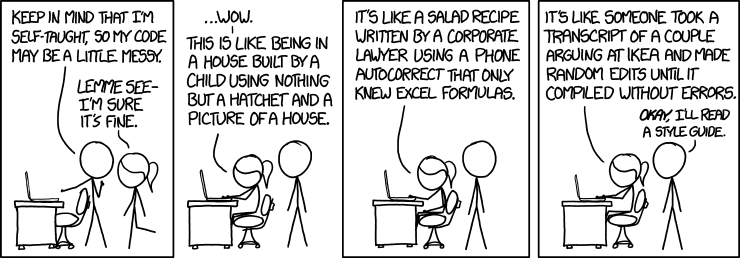
\includegraphics[width=12cm]{code_quality.png}
\caption{Following coding style guidelines is important to ensure that others may easily read, understand, and update your code. Source \textless http://xkcd.com/1513/\textgreater.}
}
\end{center}
\end{figure}

\subsection{\label{sec:level1}Code Commenting}

Every line of code should be fully documented so that any person reading the code will immediately understand what a line of code is doing within the structure of the total code.  This even includes any lines of code that seem to perform an obvious task.  If a line of code just increments some counting variable by one, then there should still be a comment saying explicitly that that is what is being done.  In this case the developer should be explicitly state what is being incremented and why it is being incremented.  For example

\begin{lstlisting}
	# This increments the camera index by 
	# one to address the next camera
	camera_index += 1
\end{lstlisting}

this case explicitly states what is being incremented and why it is being incremented.

If a line of code does something relatively complicated, then the line of code should be split into multiple lines with easier to explain comments.� Or if a line of code has to do something complicated and ugly (perhaps to save memory), then there needs to be a small paragraph of comments before the line of code saying exactly what it is doing and why it was not split up into several shorter lines of code.

If a line of code uses a ``strange" or uncommon function for some reason (ie using ``bsxfun" instead of ``repmat" in Matlab), the comments need to explain why the code does this so that a future developer doesn't later change the code back.

Additionally the comments need to be updated any time that a line of code is updated or changed; comments that explain something incorrectly are even less useful than a lack of any comments.

Algorithms in code may be commented by a block of comments in a paragraph format.  This is particularly useful if a relatively complicated (or otherwise difficult to interpret) algorithm is written into the code.  Block comments are often used to separate different portions of a code into specific sections that deal with different tasks.

\subsection{\label{sec:level1}Function Documentation}

Every function should be fully documented.� The header of the functions (the function docstring in Python jargon) should contain a list of every input and output variable and descriptions of these variables.  The description should contain a a short summary of what the variable is used for and what the variable contains.  Additionally the description should list the type of the variable, the class of the variable, and the relative size of the variable.  The variable type is based upon what data the variable contains and is typically one of the following: integer, float, string, boolean, et cetera.  The class of the variable is generally defined by how the variable was created and may be a list, a string, a tuple, an ndarray, or any other of a large number of possible classes.

The relative size of the variable should be defined by one of two possible methods.  If the size of the variable will always be constant regardless of the function input, then the size should be defined as a numerical value.  For example, the variable `{\fontfamily{pcr}\selectfont window\_resolution}' will always being a list with three elements and thus should have a size of `3'.  However if the size of the variable may differ among different function calls, then the relative size should be defined by a list of sizes equal to the number of dimensions in the variable.  For example, the size of the variable `{\fontfamily{pcr}\selectfont image\_window}' may be different each time the PIV code is called and thus should have the size defined as `MxNxP'.  If there are multiple variables with unknown sizes that may be different, then the size should be define by a different set of letters.  This way, the user will always know the relative sizes of the different variables and may get an intuitive sense about how the variables relate to one-another.

The function documentation should also list any Python modules that need to be imported to run the function and where these modules may be found.  This important to ensure that function dependencies are obvious to developers.  If there is a dependency error, then this will make it easier for developers to track down the missing dependency.

Finally, the function documentation should explicitly state what algorithm is being used and what reference (the journal paper, textbook, et cetera) was used to develop the algorithm.  The header may also contain the author or authors of the function, the date or time span over which the function was created, and whether the function was based upon a previous function or other code.  If the function was developed over time and there are several versions of the function, the comments should also state which version the function is and how the current version differs from previous versions.  An example of properly documented Python function is shown below.

\begin{lstlisting}
def calculate_window_correlation(
        image_window_1, image_window_2, window_apodization_filter,
        window_spectral_filter, window_size, correlation_method ):
            """This calculates the cross-correlation of two image windows.

            This function applies the apodization filter given by 
            window_apodization_filter to the two image windows given by 
            image_window_1 and image_window_2 and then calculates a cross-
            correlation using the method defined by correlation_method.  The 
            filter given by window_spectral_filter is then applied to the 
            cross-correlation in the Fourier domain.  An inverse DFT is then 
            applied to the cross-correlation which is then returned by this 
            function.
           
            ###################################################################
            # Input Variables                                                 #
            ###################################################################
           
            Variables                       Description
           
            image_window_1                  The window extracted from the first
                                            image. (float, ndarray, MxNxP)
                                           
            image_window_2                  The window extracted from the 
                                            second image. (float, ndarray, 
                                            MxNxP)
                                            
            window_apodization_filter       The apodization filter to apply to 
                                            the windows. (float, ndarray, 
                                            MxNxP)
                                            
            window_spectral_filter          The spectral filter to apply to 
                                            the cross-correlation in the DFT 
                                            domain. (float, ndarray, MxNxP)
                                            
            window_size                     A list of the window sizes in each 
                                            of the three dimensions. (integer, 
                                            list, 3)
                                            
            correlation_method              A string specifying the cross 
                                            correlation method to use.  The 
                                            possible values of the variable 
                                            are SCC, RPC, GCC, SPC, DCC, or 
                                            FMC. (string, string, Q)
                                            
            ###################################################################
            # Output Variables                                                #
            ###################################################################
                                            
            Variables                       Description
            
            cross_correlation               The cross-correlation of the two 
                                            windows calculated using the 
                                            specified method. (float, ndarray,
                                            MxNxP)
                                            
            ###################################################################
            # Function Dependencies                                           #
            ###################################################################
                                           
            Python Standard Modules:
            
                math
                
            Python Specialized Modules:    
                
                numpy
                scipy
                
            Python In-house Modules:
            
                standard_cross_correlation
                robust_phase_correlation
                generalized_cross_correlation
                spectral_phase_correlation
                direct_cross_correlation
                fourier_mellon_cross_correlation            
                                            
            ###################################################################
            # Function Information                                            #
            ###################################################################
                                            
            This function is based upon the Matlab function 
            calculate_window_correlation which is contained within the main 
            Matlab function piv_3d_10.  This function directly output the 
            velocity vector and only let the user select the SCC or RPC cross-
            correlation methods.
            
            Authors: Rod La Foy (rlafoy@vt.edu)
            First Created On: 7 April 2015
            Last Modified On: 7 April 2015
            
            """
\end{lstlisting}

Due to the way that Python generates documentation and help file, the function comments need to be written in a precise format.  This will ensure that future developers working on the PIV code project can easily use and build upon other developer's code.  A list of general requirements for the function docstrings is given below.

\begin{enumerate}[leftmargin=1cm,rightmargin=1cm]
	\item A function docstring is indented from the function name by four spaces.
	\item A function docstring starts with three double-quotes.
	\item The first line of the docstring is a single sentence description of the function.
	\item A blank line follows the first line in a docstring.
	\item An extensive function documentation follows the first line and blank line.
	\item A blank line follows the extensive documentation.
	\item The function docstring is ended with three double-quotes.
\end{enumerate}

A good guideline for writing function comments is that another developer on the project must be able to look at any function and tell anyone else working on the project exactly what that function's inputs and outputs are (what the variables do, what class the variables are, what dimensions the variables are, and what the function is doing with them) and what the function's dependencies are within a minute.  If this is not possible, then the function needs to be more fully documented.

\subsection{\label{sec:level1}Variables}

Variable names should be consistent and obvious (what the variable contains and what it will be used for) throughout all functions of the project code.  The following guideline should be used when creating new variables.

\begin{enumerate}[leftmargin=1cm,rightmargin=1cm]
	\item Variable names should consist of lowercase characters and underscores.  A possible variable name would be `{\fontfamily{pcr}\selectfont window\_resolution}'.
	\item Variable names should be descriptive and make it obvious to developers where the variable will be used and what it contains.  An example of a good variable name is `{\fontfamily{pcr}\selectfont pass\_index}' while the variable name `{\fontfamily{pcr}\selectfont e}' is a poor choice.
	\item Variable names should be consistent across all functions.  For example the variable `{\fontfamily{pcr}\selectfont window\_resolution}' should be used to define the window resolution across all functions that need this value.
	\item Use variable names that are consistent with journal paper variable names (when applicable) if a particular algorithm is being copied.  For example using the variable name `{\fontfamily{pcr}\selectfont uod\_normalization\_epsilon}' would be a good name for the universal outlier detector minimum normalization level $\epsilon$ value.
	\item Single letter variable names should be avoided since it is generally unclear what the variables contains or references.
	\item Use the variables `{\fontfamily{pcr}\selectfont ii}', `{\fontfamily{pcr}\selectfont jj}', and `{\fontfamily{pcr}\selectfont kk}' to index into the first, second, and third dimensions of a three-dimensional array.  In particular use these as prefixes for two and three dimensional image coordinates.
	\item Use the variables `{\fontfamily{pcr}\selectfont x}', `{\fontfamily{pcr}\selectfont y}', and `{\fontfamily{pcr}\selectfont z}' for describing world coordinates with physical units.
\end{enumerate}

A consistent system for defining image and world coordinates and velocities should be used.  For image coordinates, both in two and three dimensions, variables indexing into the image coordinates should use the format `{\fontfamily{pcr}\selectfont ii\_image\_position}', `{\fontfamily{pcr}\selectfont jj\_image\_position}', and `{\fontfamily{pcr}\selectfont kk\_image\_position}'.  The corresponding velocity variables with units of \textit{pixels/frame} should be defined by the variables `{\fontfamily{pcr}\selectfont ii\_image\_velocity}', `{\fontfamily{pcr}\selectfont jj\_image\_velocity}', and `{\fontfamily{pcr}\selectfont kk\_image\_velocity}'.  The prefix `{\fontfamily{pcr}\selectfont ii}' should always refer to indexing into the first dimension of a multi-dimensional array.  Similarly the prefix `{\fontfamily{pcr}\selectfont jj}' should always refer to indexing into the second dimension and the prefix `{\fontfamily{pcr}\selectfont jj}' should always refer to indexing into the third dimension.

A similar system is used for world coordinates to maintain consistency.  The variables defined as `{\fontfamily{pcr}\selectfont x\_world\_position}', `{\fontfamily{pcr}\selectfont y\_world\_position}', and `{\fontfamily{pcr}\selectfont z\_world\_position}' should always be used to describe world coordinates with physical units (that are defined by the user).  The physical velocity values are defined by the variables `{\fontfamily{pcr}\selectfont x\_world\_velocity}', `{\fontfamily{pcr}\selectfont y\_world\_velocity}', and `{\fontfamily{pcr}\selectfont z\_world\_velocity}'.  The velocity field that is output from the PIV code may have units in terms of image coordinates (\textit{pixels/frame}) or in terms of world coordinates (\textit{m/s}) depending upon the application.  The units that are used are also saved in the output data file.  Be default the units should be in \textit{pixels/frame} unless otherwise specified by the user.

Often it is useful to group related variable names by using a constant prefix on the variable names.  For example all the variables related to the universal outlier detector (UOD) algorithm could be in the form `{\fontfamily{pcr}\selectfont uod\_some\_name}'. This makes it easy to identify what these variables contain, what the variables are used for, and which variables need to be passed into a particular function.  A similar naming scheme may be used with suffixes instead such as `{\fontfamily{pcr}\selectfont some\_name\_uod}', however this decreases the readability of the code and is therefore not advised.

When variables are passed into a function, the document string of the function should explicitly identify each variable that is passed into the function, what class the variable is, what size the variable is, and what the variable contains.

The following tables give several variable names that should be used throughout the PIV code.  These tables are not exhaustive and may be subject to change, but should be used as a first reference when writing new functions.  The tables were primarily drawn from the `piv\_3d\_10' code.  The variable names given here mostly follow the rules specified above, but could be improved in some cases.  There are many other variables associated with PIV code that are not described in the tables, but many may be found in the `piv\_3d\_10' code.  In some cases the variable names given in `piv\_3d\_10' do not follow the conventions described in this document and should be improved.

Additionally there is a table that lists some abbreviations of common PIV code related terms.  Abbreviations should be used any time that they will improve the readability of the code (perhaps by making really long variable names shorter).  However, abbreviations may also decrease the readability of the code since the variable names are no longer explicit and the expanded form of short abbreviations is not necessarily obvious.  If abbreviations are used in the code, they should be used consistently among all functions.  For example any function that calls a deformation based variable should either use `{\fontfamily{pcr}\selectfont deformation}' or `{\fontfamily{pcr}\selectfont deform}' in all functions.  Abbreviations that are ambiguous in any way should be avoided.  For example if a function uses two variables where one refers to `option' and another refers to `optimal', then the abbreviation `{\fontfamily{pcr}\selectfont opt}' should not be used in this function.

% This changes the margins of the current page to ensure that the table fits well
\newgeometry{a4paper,left=1in,right=1in,top=1in,bottom=1in,nohead}

% Ensure that the commands only apply to the current page
\afterpage{

	%%%%%%%%%%%%%%%%%%%%%%%%%%%%%%%%%%%%%%%%%%%%%%%%%%%%%%%%%%%%%%%%%%%%%%%%%
	% General Processing Parameter Variables                                %
	%%%%%%%%%%%%%%%%%%%%%%%%%%%%%%%%%%%%%%%%%%%%%%%%%%%%%%%%%%%%%%%%%%%%%%%%%

	% Flush earlier floating objects (otherwise order might not be correct)
    \clearpage
    % Empty page style (ie no header or footer space)
    \thispagestyle{empty}
    % Format the current page in landscape
    \begin{landscape}
        % Center the table
        \centering
         
        % This puts the table in a box to make the centering work better (I don't know why this is necessary)
        \makebox[0pt]{
        
	        % Make the spacing in the table a little larger for easier readability
	       	\setlength{\arrayrulewidth}{1pt}
			\renewcommand{\arraystretch}{1.15}
			
			% Start the table object
			\begin{tabular}{ l l l l l }
				% Insert a thick top line
				\toprule
				% Insert the table title
	  			\multicolumn{5}{ c }{General Processing Input Parameters} \\
				% Insert a thinner middle line
				\midrule
	  			Name 															& Type 		& Size 	& Possible Values 						& Description	\\
	  			% Insert a thinner middle line
				\midrule
	  			{\fontfamily{pcr}\selectfont image\_read\_directory}				& String 	& M	 	& `/mnt/stuff/' 							& Directory containing PIV images.						\\
	  			{\fontfamily{pcr}\selectfont image\_filename\_prefix} 				& String		& N		& `frame\_'								& PIV image filename prefix.								\\
	  			{\fontfamily{pcr}\selectfont image\_filename\_extension}			& String		& P		& `tif', `jpg', `mat', `h5', et cetera	& PIV image filename extension.							\\
	  			{\fontfamily{pcr}\selectfont image\_variable\_name}				& String		& Q		& `I', Null, et cetera					& Variable name within data structure (if applicable).		\\
	  																			&			&		&										&														\\
			  	{\fontfamily{pcr}\selectfont vector\_field\_write\_directory}		& String		& R		& `/mnt/morestuff/'						& Directory in which to write the velocity vectors.		\\
			    																	&			&		&										&														\\
			 	{\fontfamily{pcr}\selectfont initial\_image\_frame}				& Integer	& 1		& 1										& Index into image numbers to start processing.			\\
				{\fontfamily{pcr}\selectfont final\_image\_frame}					& Integer	& 1		& 2										& Index into image numbers to finish processing.			\\
				{\fontfamily{pcr}\selectfont image\_frame\_step}					& Integer	& 1		& 1										& Image numbers to skip between frame pairs.				\\
				{\fontfamily{pcr}\selectfont image\_correlation\_step}				& Integer	& 1		& 1										& Image index separation between correlation pairs.		\\
																				&			&		&										&														\\
				{\fontfamily{pcr}\selectfont pass\_number}							& Integer	& 1		& 3										& Number of cross-correlation passes to perform.			\\
																				&			&		&										&														\\
				{\fontfamily{pcr}\selectfont par\_process\_perform}				& Boolean	& 1		& True, False							& Defines whether to use multiple cores during processing.	\\
				{\fontfamily{pcr}\selectfont par\_process\_node\_number}			& Integer	& 1		& 4										& Number of processors to use during processing.			\\
																				&			&		&										&														\\
				{\fontfamily{pcr}\selectfont window\_deform\_perform}				& Boolean	& 1		& True, False							& Defines whether to perform window deformation.			\\
				{\fontfamily{pcr}\selectfont window\_deform\_iter\_min}			& Integer	& 1		& 1										& Minimum number of window deformation iterations.			\\
				{\fontfamily{pcr}\selectfont window\_deform\_iter\_max}			& Integer	& 1		& 5										& Maximum number of window deformation iterations.			\\
				{\fontfamily{pcr}\selectfont window\_deform\_thresh}				& Float		& 1		& 0.5									& Deformation convergence threshhold.						\\
				% Insert a thick bottom line
				\bottomrule
			\end{tabular}
		}

    \end{landscape}
    
    \clearpage
    
    	%%%%%%%%%%%%%%%%%%%%%%%%%%%%%%%%%%%%%%%%%%%%%%%%%%%%%%%%%%%%%%%%%%%%%%%%%
	% Pass Specific Processing Parameter Variables                          %
	%%%%%%%%%%%%%%%%%%%%%%%%%%%%%%%%%%%%%%%%%%%%%%%%%%%%%%%%%%%%%%%%%%%%%%%%%
    
    % Flush earlier floating objects (otherwise order might not be correct)
    \clearpage
    % Empty page style (ie no header or footer space)
    \thispagestyle{empty}
    % Format the current page in landscape
    \begin{landscape}
        % Center the table
        \centering
         
        % This puts the table in a box to make the centering work better (I don't know why this is necessary)
        \makebox[0pt]{
        
	        % Make the spacing in the table a little larger for easier readability
	       	\setlength{\arrayrulewidth}{1pt}
			\renewcommand{\arraystretch}{1.15}
			
			% Start the table object
			\begin{tabular}{ l l l l l }
				% Insert a thick top line
				\toprule
				% Insert the table title
	  			\multicolumn{5}{ c }{Pass Specific Processing Input Parameters} \\
				% Insert a thinner middle line
				\midrule
	  			Name 															& Type 		& Size 	& Possible Values 						& Description	\\
	  			% Insert a thinner middle line
				\midrule
	  			{\fontfamily{pcr}\selectfont pass\_index}							& Integer 	& 1	 	& 1 										& The index of the current PIV pass.						\\
	  																			&			&		&										&														\\
				{\fontfamily{pcr}\selectfont window\_resolution}	 				& Integer	& 3		& [64,64,64]								& The effective window resolution after windowing.			\\
	  			{\fontfamily{pcr}\selectfont window\_size}							& Integer	& 3		& [128,128,128]							& The window array dimensions.							\\
	  			{\fontfamily{pcr}\selectfont window\_gridding\_method}				& String		& M		& `window\_overlap', `window\_spacing'	& Method used to calculate the window coordinates.			\\
			  	{\fontfamily{pcr}\selectfont window\_overlap}						& Float		& 3		& [0.5,0.5,0.5]							& The ratio of the adjacent window overlap distances.		\\
			 	{\fontfamily{pcr}\selectfont window\_spacing}						& Integer	& 3		& [64,64,64]								& The distance between adjacent windows.					\\
	  																			&			&		&										&														\\
				{\fontfamily{pcr}\selectfont bulk\_window\_offset}					& Float		& 3		& [0,0,0]								& A specified initial window displacement.					\\
					  															&			&		&										&														\\
				{\fontfamily{pcr}\selectfont correlation\_method}					& String		& N		& 'RPC', 'SCC', 'DCC', et cetera			& The method used to perform the cross-correlation.		\\
																				&			&		&										&														\\
				{\fontfamily{pcr}\selectfont zero\_mean\_windows}					& Boolean	& 1		& True, False							& Defines whether to subtract window mean from windows.	\\
																				&			&		&										&														\\
				{\fontfamily{pcr}\selectfont validate\_vector\_field}				& Boolean	& 1		& True, False							& Perform validation on measured velocity field.			\\
																				&			&		&										&														\\
				{\fontfamily{pcr}\selectfont min\_outlier\_thresh}		& Float		& 3		& [-8,-8,-8]								& Minimum velocity below which is considered an outlier.	\\
				{\fontfamily{pcr}\selectfont max\_outlier\_thresh}		& Float		& 3		& [+8,+8,+8]								& Maximum velocity below which is considered an outlier.	\\
																				&			&		&										&														\\
				{\fontfamily{pcr}\selectfont uod\_kernal\_size}					& Integer	& 3		& [3,3,3]								& UOD validation array dimensions.						\\
				{\fontfamily{pcr}\selectfont uod\_epsilon}							& Float		& 1		& 0.1									& UOD validation epsilon value.							\\
				{\fontfamily{pcr}\selectfont uod\_residual\_thresh}			& Float		& 1		& 1.5									& UOD validation threshhold value.						\\
																				&			&		&										&														\\
				{\fontfamily{pcr}\selectfont vector\_replacement\_method}			& String		& P		& `median', `laplacian', `delaunay'		& Method used to interpolate invalid velocity vectors.		\\
				{\fontfamily{pcr}\selectfont median\_valid\_vector\_number}		& Integer	& 1		& 8										& Minimum number of valid vectors to perform replacement.	\\
				{\fontfamily{pcr}\selectfont laplacian\_adjacent\_connectivity}		& Integer	& 1		& 4										& Connectivity of adjacent vectors for replacement.		\\
				{\fontfamily{pcr}\selectfont delaunay\_interpolation\_weighting}	& String		& Q		& `natural', `linear', `nearest'			& Weighting method for vector replacement.					\\
																				&			&		&										&														\\
				{\fontfamily{pcr}\selectfont smooth\_vector\_field	}				& Boolean	& 1		& True, False							& Whether to perform velocity field smoothing.				\\
				{\fontfamily{pcr}\selectfont gaussian\_smoothing\_kernal\_std}		& Float		& 1		& 1										& Standard deviation of Gaussian smoothing kernal.			\\
				{\fontfamily{pcr}\selectfont gaussian\_smoothing\_kernal\_size}		& Integer	& 3		& [7,7,7]								& Size of Gaussian smoothing kernal.						\\

				% Insert a thick bottom line
				\bottomrule
			\end{tabular}
		}

    \end{landscape}
    
    \clearpage
    
    %%%%%%%%%%%%%%%%%%%%%%%%%%%%%%%%%%%%%%%%%%%%%%%%%%%%%%%%%%%%%%%%%%%%%%%%%
	% PIV Processing Output Parameters 			                          %
	%%%%%%%%%%%%%%%%%%%%%%%%%%%%%%%%%%%%%%%%%%%%%%%%%%%%%%%%%%%%%%%%%%%%%%%%%
    
    % Flush earlier floating objects (otherwise order might not be correct)
    \clearpage
    % Empty page style (ie no header or footer space)
    \thispagestyle{empty}
    % Format the current page in landscape
    \begin{landscape}
        % Center the table
        \centering
         
        % This puts the table in a box to make the centering work better (I don't know why this is necessary)
        \makebox[0pt]{
        
	        % Make the spacing in the table a little larger for easier readability
	       	\setlength{\arrayrulewidth}{1pt}
			\renewcommand{\arraystretch}{1.15}
			
			% Start the table object
			\begin{tabular}{ l l l l l }
				% Insert a thick top line
				\toprule
				% Insert the table title
	  			\multicolumn{5}{ c }{PIV Processing Output Data} \\
				% Insert a thinner middle line
				\midrule
	  			Name 															& Type 		& Size 	& Possible Values 						& Description	\\
	  			% Insert a thinner middle line
				\midrule
	  			{\fontfamily{pcr}\selectfont pass\_index}							& Integer 	& 1 		& 1 										& The index of the current PIV pass.						\\
	  																			&			&		&										&														\\
				{\fontfamily{pcr}\selectfont vector\_geometry}		 				& String		& M		& `gridded', `scattered'					& The geometric arrangement of the velocity vectors.		\\
				{\fontfamily{pcr}\selectfont vector\_grid\_size}		 			& Integer	& 3		& [100,100,25], Null						& The size of the (gridded) window vector array.			\\
	  																			&			&		&										&														\\
				{\fontfamily{pcr}\selectfont x\_world\_position}		 			& Float		& N		& [0,1,2,...]							& The X dimension window coordinates.						\\
				{\fontfamily{pcr}\selectfont y\_world\_position}		 			& Float		& N		& [3,4,5,...]							& The Y dimension window coordinates.						\\
				{\fontfamily{pcr}\selectfont z\_world\_position}		 			& Float		& N		& [6,7,8,...]							& The Z dimension window coordinates.						\\
				{\fontfamily{pcr}\selectfont units\_world\_position}		 		& String		& P		& `pixel', `m', `mm', et cetera			& The window coordinates units.							\\
	  																			&			&		&										&														\\
				{\fontfamily{pcr}\selectfont x\_world\_velocity}		 			& Float		& N		& [0.0,1.1,2.2,...]						& The X dimension (U) window velocity values.				\\
				{\fontfamily{pcr}\selectfont y\_world\_velocity}		 			& Float		& N		& [3.3,4.4,5.5,...]						& The Y dimension (V) window velocity values.				\\
				{\fontfamily{pcr}\selectfont z\_world\_velocity}		 			& Float		& N		& [6.6,7.7,8.8,...]						& The Z dimension (W) window velocity values.				\\
				{\fontfamily{pcr}\selectfont units\_world\_velocity}		 		& String		& Q		& `pixel/frame', `m/s', `mm/s', et cetera	& The window velocity units.								\\

	  																			&			&		&										&														\\
				{\fontfamily{pcr}\selectfont x\_velocity\_uncertainty}		 		& Float		& N		& [0.1,0.2,0.1,...]						& The X dimension (U) window velocity uncertainty values.	\\
				{\fontfamily{pcr}\selectfont y\_velocity\_uncertainty}		 		& Float		& N		& [0.2,0.1,0.2,...]						& The Y dimension (V) window velocity uncertainty values.	\\
				{\fontfamily{pcr}\selectfont z\_velocity\_uncertainty}		 		& Float		& N		& [0.3,0.2,0.2,...]						& The Z dimension (W) window velocity uncertainty values.	\\
	  																			&			&		&										&						  								\\
				{\fontfamily{pcr}\selectfont vector\_replaced}						& Boolean	& N		& True, False							& Whether velocity vector replaced during validation.		\\
				% Insert a thick bottom line
				\bottomrule
			\end{tabular}
		}

    \end{landscape}
    
    \clearpage
    
    %%%%%%%%%%%%%%%%%%%%%%%%%%%%%%%%%%%%%%%%%%%%%%%%%%%%%%%%%%%%%%%%%%%%%%%%%
	% General PIV Code Variables      			                          %
	%%%%%%%%%%%%%%%%%%%%%%%%%%%%%%%%%%%%%%%%%%%%%%%%%%%%%%%%%%%%%%%%%%%%%%%%%
    
    % Flush earlier floating objects (otherwise order might not be correct)
    \clearpage
    % Empty page style (ie no header or footer space)
    \thispagestyle{empty}
    % Format the current page in landscape
    \begin{landscape}
        % Center the table
        \centering
         
        % This puts the table in a box to make the centering work better (I don't know why this is necessary)
        \makebox[0pt]{
        
	        % Make the spacing in the table a little larger for easier readability
	       	\setlength{\arrayrulewidth}{1pt}
			\renewcommand{\arraystretch}{1.15}
			
			% Start the table object
			\begin{tabular}{ l l l l l }
				% Insert a thick top line
				\toprule
				% Insert the table title
	  			\multicolumn{5}{ c }{General PIV Code Variables} \\
				% Insert a thinner middle line
				\midrule
	  			Name 															& Type 		& Size 		& Possible Values 						& Description	\\
	  			% Insert a thinner middle line
				\midrule
	  			{\fontfamily{pcr}\selectfont image\_size}							& Integer 	& 3	 		& [1024,1024,256] 						& The size of the PIV image array.										\\
	  																			&			&			&										&																		\\
				{\fontfamily{pcr}\selectfont ii\_window\_position}		 			& Float		& M			& [0,1,2,...]							& The 1\textsuperscript{st} dimension window coordinates.					\\
				{\fontfamily{pcr}\selectfont jj\_window\_position}		 			& Float		& M			& [3,4,5,...]							& The 2\textsuperscript{nd} dimension window coordinates.					\\
				{\fontfamily{pcr}\selectfont kk\_window\_position}		 			& Float		& M			& [6,7,8,...]							& The 3\textsuperscript{rd} dimension window coordinates.					\\
	  																			&			&			&										&																		\\
				{\fontfamily{pcr}\selectfont ii\_window\_displacement}		 		& Float		& M			& [0.0,1.1,2.2,...]						& The 1\textsuperscript{st} dimension window velocity values.				\\
				{\fontfamily{pcr}\selectfont jj\_window\_displacement}		 		& Float		& M			& [3.3,4.4,5.5,...]						& The 2\textsuperscript{nd} dimension window velocity values.				\\
				{\fontfamily{pcr}\selectfont kk\_window\_displacement}		 		& Float		& M			& [6.6,7.7,8.8,...]						& The 3\textsuperscript{rd} dimension window velocity values.				\\
	  																			&			&			&										&																		\\
				{\fontfamily{pcr}\selectfont ii\_window\_displacement\_uncertainty}	& Float		& M			& [0.1,0.2,0.1,...]						& The 1\textsuperscript{st} dimension window velocity uncertainty values.	\\
				{\fontfamily{pcr}\selectfont jj\_window\_displacement\_uncertainty}	& Float		& M			& [0.2,0.1,0.2,...]						& The 2\textsuperscript{nd} dimension window velocity uncertainty values.	\\
				{\fontfamily{pcr}\selectfont kk\_window\_displacement\_uncertainty}	& Float		& M			& [0.3,0.2,0.2,...]						& The 3\textsuperscript{rd} dimension window velocity uncertainty values.	\\
	  																			&			&			&										&						  												\\
				{\fontfamily{pcr}\selectfont outlier\_vector\_array}				& Boolean	& M			& True, False							& Whether velocity vector is identified as an outlier.						\\
	  																			&			&			&										&						  												\\
				{\fontfamily{pcr}\selectfont rpc\_spectral\_filter}				& Float		& NxPxQ		& [[0.1,0.2,0.3,...]]						& The RPC spectral energy filter.											\\
				{\fontfamily{pcr}\selectfont window\_apodization\_filter}			& Float		& NxPxQ		& [[0.1,0.2,0.3,...]]						& The correlation window apodization filter.								\\
	  																			&			&			&										&						  												\\
				{\fontfamily{pcr}\selectfont image\_frames}						& Float		& SxTxUxV	& [[0.1,0.2,0.3,...]]						& An array of the current image frames to process.							\\
	  																			&			&			&										&						  												\\
				{\fontfamily{pcr}\selectfont image\_windows}						& Float		& NxPxQxR	& [[0.1,0.2,0.3,...]]						& An array of windows extracted from the current images.					\\
				{\fontfamily{pcr}\selectfont image\_dft\_windows}					& Float		& NxPxQxR	& [[0.1,0.2,0.3,...]]						& The DFT of the windows extracted from the current images.				\\
	  																			&			&			&										&						  												\\
				{\fontfamily{pcr}\selectfont cross\_correlation}					& Float		& NxPxQ		& [[0.1,0.2,0.3,...]]						& The cross-correlation of the current window pair.						\\

				% Insert a thick bottom line
				\bottomrule
			\end{tabular}
		}

    \end{landscape}
    
    \clearpage
    
    %%%%%%%%%%%%%%%%%%%%%%%%%%%%%%%%%%%%%%%%%%%%%%%%%%%%%%%%%%%%%%%%%%%%%%%%%
	% PIV Code Abbreviations		      			                          %
	%%%%%%%%%%%%%%%%%%%%%%%%%%%%%%%%%%%%%%%%%%%%%%%%%%%%%%%%%%%%%%%%%%%%%%%%%
    
    % Flush earlier floating objects (otherwise order might not be correct)
    \clearpage
    % Empty page style (ie no header or footer space)
    \thispagestyle{empty}
    % Format the current page in landscape
    \begin{landscape}
        % Center the table
        \centering
         
        % This puts the table in a box to make the centering work better (I don't know why this is necessary)
        \makebox[0pt]{
        
	        % Make the spacing in the table a little larger for easier readability
	       	\setlength{\arrayrulewidth}{1pt}
			\renewcommand{\arraystretch}{1.15}
			
			% Start the table object
			\begin{tabular}{ l l l }
				% Insert a thick top line
				\toprule
				% Insert the table title
	  			\multicolumn{3}{ c }{PIV Code Abbreviations} \\
				% Insert a thinner middle line
				\midrule
	  			Full Word or Phrase 					& Code Abbreviation 									& Description													\\
	  			% Insert a thinner middle line
				\midrule
				particle image velocimetry			& {\fontfamily{pcr}\selectfont piv}					& Particle Image Velocimetry methodology.							\\
				particle tracking velocimetry			& {\fontfamily{pcr}\selectfont ptv}					& Particle Tracking Velocimetry methodology.						\\						
				stereographic						& {\fontfamily{pcr}\selectfont stereo}				& Any stereographic operation.									\\				
				tomography							& {\fontfamily{pcr}\selectfont tomo}					& Any tomographic operation.										\\
				calibration							& {\fontfamily{pcr}\selectfont cal}					& Any calibration operation.										\\
				camera								& {\fontfamily{pcr}\selectfont cam}					& Any camera related operation.									\\
													&													&																\\
				directory							& {\fontfamily{pcr}\selectfont dir}					& Any computer directory.											\\
				image								& {\fontfamily{pcr}\selectfont im}					& Any two or three dimensional image.								\\
													&													&																\\
				deformation							& {\fontfamily{pcr}\selectfont deform}				& Window deformation technique.									\\
				coordinates							& {\fontfamily{pcr}\selectfont coord}					& Any image or world coordinates.									\\
				velocity								& {\fontfamily{pcr}\selectfont vel}					& Any velocity values.											\\
				vector								& {\fontfamily{pcr}\selectfont vect}					& Any arbitrary dimensional vector.								\\
													&													&																\\
				interpolation						& {\fontfamily{pcr}\selectfont interp}				& An interpolation function or interpolated value.					\\
				minimum								& {\fontfamily{pcr}\selectfont min}					& A minimum value of some set.									\\
				maximum								& {\fontfamily{pcr}\selectfont max}					& A maximum value of some set.									\\
				optimum								& {\fontfamily{pcr}\selectfont opt}					& An optimal value of some set.									\\
				threshhold							& {\fontfamily{pcr}\selectfont thresh}				& A cutoff threshhold value for dividing a set.					\\
				gaussian								& {\fontfamily{pcr}\selectfont gauss}					& A Gaussian function.											\\		
				standard deviation					& {\fontfamily{pcr}\selectfont std}					& The standard deviation of some set.								\\
				discrete fourier transform			& {\fontfamily{pcr}\selectfont dft}					& The Discrete Fourier Transform of a vector.						\\
				fast fourier transform				& {\fontfamily{pcr}\selectfont fft}					& The Fast Fourier Transform of a vector.							\\
				number								& {\fontfamily{pcr}\selectfont num}					& Any number for any reason.										\\
				residual								& {\fontfamily{pcr}\selectfont res}					& The residual of some operation.									\\
				radius								& {\fontfamily{pcr}\selectfont rad}					& The radius from some point in some metric.						\\
				%									&													&																\\
				%standard cross correlation			& {\fontfamily{pcr}\selectfont scc}					& The standard cross-correlation of two functions.					\\
				%robust phase correlation				& {\fontfamily{pcr}\selectfont rpc}					& The robust phase correlation of two functions.					\\	
				%generalized cross correlation			& {\fontfamily{pcr}\selectfont gcc}					& The generalized cross-correlation of two functions.				\\
				%spectral phase correlation			& {\fontfamily{pcr}\selectfont spc}					& The spectral phase correlation of two functions.					\\
				%direct cross correlation				& {\fontfamily{pcr}\selectfont dcc}					& The direct cross-correlation of two functions.					\\
				%fourier mellin cross correlation		& {\fontfamily{pcr}\selectfont fmc}					& The Fourier-Mellin Transform cross-correlation of two functions.	\\
				% Insert a thick bottom line
				\bottomrule
			\end{tabular}
		}

    \end{landscape}
    
    \clearpage
    
    % Flush earlier floating objects (otherwise order might not be correct)
    \clearpage
    % Empty page style (ie no header or footer space)
    \thispagestyle{empty}
    % Format the current page in landscape
    \begin{landscape}
        % Center the table
        \centering
         
        % This puts the table in a box to make the centering work better (I don't know why this is necessary)
        \makebox[0pt]{
        
	        % Make the spacing in the table a little larger for easier readability
	       	\setlength{\arrayrulewidth}{1pt}
			\renewcommand{\arraystretch}{1.15}
			
			% Start the table object
			\begin{tabular}{ l l l }
				% Insert a thick top line
				\toprule
				% Insert the table title
	  			\multicolumn{3}{ c }{PIV Code Abbreviations Continued} \\
				% Insert a thinner middle line
				\midrule
	  			Full Word or Phrase 					& Code Abbreviation 									& Description													\\
	  			% Insert a thinner middle line
				\midrule
				%particle image velocimetry			& {\fontfamily{pcr}\selectfont piv}					& Particle Image Velocimetry methodology.							\\
				%particle tracking velocimetry			& {\fontfamily{pcr}\selectfont ptv}					& Particle Tracking Velocimetry methodology.						\\						
				%stereographic						& {\fontfamily{pcr}\selectfont stereo}				& Any stereographic operation.									\\				
				%tomography							& {\fontfamily{pcr}\selectfont tomo}					& Any tomographic operation.										\\
				%calibration							& {\fontfamily{pcr}\selectfont cal}					& Any calibration operation.										\\
				%camera								& {\fontfamily{pcr}\selectfont cam}					& Any camera related operation.									\\
				%									&													&																\\
%				directory							& {\fontfamily{pcr}\selectfont dir}					& Any computer directory.											\\
%				image								& {\fontfamily{pcr}\selectfont im}					& Any two or three dimensional image.								\\
%													&													&																\\
%				deformation							& {\fontfamily{pcr}\selectfont deform}				& Window deformation technique.									\\
%				coordinates							& {\fontfamily{pcr}\selectfont coord}					& Any image or world coordinates.									\\
%				velocity								& {\fontfamily{pcr}\selectfont vel}					& Any velocity values.											\\
%				vector								& {\fontfamily{pcr}\selectfont vect}					& Any arbitrary dimensional vector.								\\
%													&													&																\\
%				interpolation						& {\fontfamily{pcr}\selectfont interp}				& An interpolation function or interpolated value.					\\
%				minimum								& {\fontfamily{pcr}\selectfont min}					& A minimum value of some set.									\\
%				maximum								& {\fontfamily{pcr}\selectfont max}					& A maximum value of some set.									\\
%				optimum								& {\fontfamily{pcr}\selectfont opt}					& An optimal value of some set.									\\
%				threshhold							& {\fontfamily{pcr}\selectfont thresh}				& A cutoff threshhold value for dividing a set.					\\
%				gaussian								& {\fontfamily{pcr}\selectfont gauss}					& A Gaussian function.											\\		
%				standard deviation					& {\fontfamily{pcr}\selectfont std}					& The standard deviation of some set.								\\
%				discrete fourier transform			& {\fontfamily{pcr}\selectfont dft}					& The Discrete Fourier Transform of a vector.						\\
%				fast fourier transform				& {\fontfamily{pcr}\selectfont fft}					& The Fast Fourier Transform of a vector.							\\
%				number								& {\fontfamily{pcr}\selectfont num}					& Any number for any reason.										\\
%				residual								& {\fontfamily{pcr}\selectfont res}					& The residual of some operation.									\\
%				radius								& {\fontfamily{pcr}\selectfont rad}					& The radius from some point in some metric.						\\
%													&													&																\\
				standard cross correlation			& {\fontfamily{pcr}\selectfont scc}					& The standard cross-correlation of two functions.					\\
				robust phase correlation				& {\fontfamily{pcr}\selectfont rpc}					& The robust phase correlation of two functions.					\\	
				generalized cross correlation			& {\fontfamily{pcr}\selectfont gcc}					& The generalized cross-correlation of two functions.				\\
				spectral phase correlation			& {\fontfamily{pcr}\selectfont spc}					& The spectral phase correlation of two functions.					\\
				direct cross correlation				& {\fontfamily{pcr}\selectfont dcc}					& The direct cross-correlation of two functions.					\\
				fourier mellin cross correlation		& {\fontfamily{pcr}\selectfont fmc}					& The Fourier-Mellin Transform cross-correlation of two functions.	\\
				% Insert a thick bottom line
				\bottomrule
			\end{tabular}
		}

    \end{landscape}
    
    \clearpage
  
}
% Reset the page geometry margins back to the normal values
\restoregeometry

\section{\label{sec:level1}General Python Coding Comments (from PEP 8)}

The following coding guidelines are generally useful Python coding rules.  These should be followed while developing the new version of Prana, but the rules are generally useful Python coding practices to follow for unrelated work.  These guidelines are drawn primarily from the PEP 8 Python coding guidelines written by Guido van Rossum, Barry Warsaw, and Nick Coghlan.

\subsection{\label{sec:level1}Function Names}

Function names should be lowercase, with words separated by underscores as necessary to improve readability.

mixedCase is allowed only in contexts where that's already the prevailing style (e.g. threading.py), to retain backwards compatibility.

\subsection{\label{sec:level1}Indentation}

Use 4 spaces per indentation level.

Continuation lines should align wrapped elements either vertically using Python's implicit line joining inside parentheses, brackets and braces, or using a hanging indent.  When using a hanging indent the following considerations should be applied; there should be no arguments on the first line and further indentation should be used to clearly distinguish itself as a continuation line.

Yes:

\begin{lstlisting}
    # Aligned with opening delimiter.
    foo = long_function_name(var_one, var_two,
                             var_three, var_four)

    # More indentation included to distinguish this from the rest.
    def long_function_name(
            var_one, var_two, var_three,
            var_four):
        print(var_one)

    # Hanging indents should add a level.
    foo = long_function_name(
        var_one, var_two,
        var_three, var_four)
\end{lstlisting}

No:

\begin{lstlisting}
    # Arguments on first line forbidden when not using vertical alignment.
    foo = long_function_name(var_one, var_two,
        var_three, var_four)

    # Further indentation required as indentation is not distinguishable.
    def long_function_name(
        var_one, var_two, var_three,
        var_four):
        print(var_one)
\end{lstlisting}

The closing brace/bracket/parenthesis on multi-line constructs may either line up under the first non-whitespace character of the last line of list, as in

\begin{lstlisting}
    my_list = [
        1, 2, 3,
        4, 5, 6,
        ]
    result = some_function_that_takes_arguments(
        'a', 'b', 'c',
        'd', 'e', 'f',
        )
\end{lstlisting}

or it may be lined up under the first character of the line that starts the multi-line construct, as in

\begin{lstlisting}
    my_list = [
        1, 2, 3,
        4, 5, 6,
    ]
    result = some_function_that_takes_arguments(
        'a', 'b', 'c',
        'd', 'e', 'f',
    )   
\end{lstlisting}

\subsection{\label{sec:level1}Tabs or Spaces}

Spaces are the preferred indentation method. Tabs should be used solely to remain consistent with code that is already indented with tabs. Python 3 disallows mixing the use of tabs and spaces for indentation. Python 2 code indented with a mixture of tabs and spaces should be converted to using spaces exclusively.

\subsection{\label{sec:level1}Maximum Line Length}

Limit all lines to a maximum of 79 characters. For flowing long blocks of text with fewer structural restrictions (docstrings or comments), the line length should be limited to 72 characters. Limiting the required editor window width makes it possible to have several files open side-by-side, and works well when using code review tools that present the two versions in adjacent columns.

The default wrapping in most tools disrupts the visual structure of the code, making it more difficult to understand. The limits are chosen to avoid wrapping in editors with the window width set to 80, even if the tool places a marker glyph in the final column when wrapping lines. Some web based tools may not offer dynamic line wrapping at all.

The Python standard library is conservative and requires limiting lines to 79 characters (and docstrings/comments to 72).

The preferred way of wrapping long lines is by using Python's implied line continuation inside parentheses, brackets and braces.  Long lines can be broken over multiple lines by wrapping expressions in parentheses. These should be used in preference to using a backslash for line continuation.

\subsection{\label{sec:level1}Blank Lines}

Separate top-level function and class definitions with two blank lines. Method definitions inside a class are separated by a single blank line.

Extra blank lines may be used (sparingly) to separate groups of related functions.  Blank lines may be omitted between a bunch of related one-liners (e.g. a set of dummy implementations). Use blank lines in functions, sparingly, to indicate logical sections.

\subsection{\label{sec:level1}Imports}

Imports should usually be on separate lines, for example

Yes: 

\begin{lstlisting}
	import os
	import sys
\end{lstlisting}

No:

\begin{lstlisting}
	import sys, os
\end{lstlisting}

It's okay to say this though:

\begin{lstlisting}
      from subprocess import Popen, PIPE
\end{lstlisting}

Imports are always put at the top of the file, just after any module comments and docstrings, and before module globals and constants. Imports should be grouped in the following order:
\begin{enumerate}
	\item standard library imports
  	\item related third party imports
	\item local application/library specific imports
\end{enumerate}

You should put a blank line between each group of imports.

Absolute imports are recommended, as they are usually more readable and tend to be better behaved (or at least give better error messages) if the import system is incorrectly configured (such as when a directory inside a package ends up on ``sys.path'').  For example the following are acceptable absolute import commands:

\begin{lstlisting}
    import mypkg.sibling
    from mypkg import sibling
    from mypkg.sibling import example
\end{lstlisting}

\subsection{\label{sec:level1}String Quotes}

In Python, single-quoted strings and double-quoted strings are the same.  The PEP documentation does not make a recommendation for this.  Pick a rule and stick to it.  When a string contains single or double quote characters, however, use the other one to avoid backslashes in the string. It improves readability.

\section{\label{sec:level1}Setting Up Python}

These are some general guidelines to be used for setting up a Python programming environment on a computer.  These guidelines do not have to be followed if the user is highly familiar with the Python programming environment, however these guidelines are highly recommended for new users.

\subsection{\label{sec:level1}Installing a Python Package Manager}

The Python package managers allow the user to easily import and update portions of the Python programming language. Additionally the package manager creates as a separate version of Python from the operating system. This ensures that updates will not potentially damage the operating system by overwriting system files.  Users are strongly recommended to use a package manager for the Python programming environment.

The following instructions are used for the installation of the Miniconda Python package manager.

Linux:
\begin{enumerate}[leftmargin=1cm,rightmargin=1cm]
	\item Go to the website \textless http://conda.pydata.org/miniconda.html\textgreater
	\item Download the Python 2.7 installer (probably `64-bit (bash installer)') to some directory such as \texttildelow /Documents/Software/
	\item Open a terminal
	\item Change the directory to where the installer was saved (`{\fontfamily{pcr}\selectfont cd \texttildelow /Documents/Software/}')
	\item Run the command `{\fontfamily{pcr}\selectfont sudo bash Miniconda-latest-Linux-x86\_64.sh}'
	\item Press `Enter' to scroll through the software license agreement
	\item Type `{\fontfamily{pcr}\selectfont yes}' and press `Enter' when prompted `{\fontfamily{pcr}\selectfont Do you approve the license terms? [yes\textbar no]}'
	\item When prompted where to install miniconda, agree to the default location by pressing `Enter'
	\item When prompted `{\fontfamily{pcr}\selectfont Do you wish the installer to prepend the Miniconda install location to PATH in your \texttildelow /bashrc \textgreater [yes\textbar no]}' type `{\fontfamily{pcr}\selectfont yes}' and press `Enter'
	\item Close the terminal and open a new terminal session (since changes to the terminal environment were made)
	\item Type `{\fontfamily{pcr}\selectfont conda update conda}' to ensure that Miniconda correctly installed and is up to date.
\end{enumerate}

OSX:
\begin{enumerate}[leftmargin=1cm,rightmargin=1cm]
	\item Go to the website \textless http://conda.pydata.org/miniconda.html\textgreater
	\item Download the Python 2.7 installer (`64-bit (bash installer)') to some directory such as \texttildelow /Documents/Software/
	\item Open a terminal
	\item Change the directory to where the installer was saved (`{\fontfamily{pcr}\selectfont cd \texttildelow /Documents/Software/}')
	\item Run the command `{\fontfamily{pcr}\selectfont sudo bash Miniconda-latest-Linux-x86\_64.sh}'
	\item Press `down-arrow' to scroll through the software license agreement
	\item Type `{\fontfamily{pcr}\selectfont yes}' and press `Enter' when prompted `{\fontfamily{pcr}\selectfont Do you approve the license terms? [yes\textbar no]}'
	\item When prompted where to install miniconda, agree to the default location by pressing `Enter'
	\item When prompted `{\fontfamily{pcr}\selectfont Do you wish the installer to prepend the Miniconda install location to PATH in your \texttildelow /bashrc \textgreater [yes\textbar no]}' type `{\fontfamily{pcr}\selectfont yes}' and press `Enter'
	\item Close the terminal and open a new terminal session (since changes to the terminal environment were made)
	\item Type `{\fontfamily{pcr}\selectfont conda update conda}' to ensure that Miniconda correctly installed and is up to date.
\end{enumerate}

\subsection{\label{sec:level1}Installing a Python Integrated Development Environment (IDE)}

The user can choose any Python IDE that he or she chooses, however to make cooperative development easier it is recommended that everyone uses the same IDE.  The Spyder IDE was chosen as a well designed Python IDE that allows the users to easily integrate writing and debugging code.  Additionally Spyder has many similarities to the Matlab desktop and as such, should present a familiar development environment to many users. The following instructions are used for the installation of the Spyder IDE.

Linux:
\begin{enumerate}[leftmargin=1cm,rightmargin=1cm]
	\item Open a terminal
	\item Type `{\fontfamily{pcr}\selectfont conda install spyder}' and press `Enter'
	\item When prompted whether to `{\fontfamily{pcr}\selectfont Proceed ([y]/n)?}' type `{\fontfamily{pcr}\selectfont y}' press 'Enter'
	\item When installation is complete, open Spyder by typing `{\fontfamily{pcr}\selectfont spyder}' and pressing `Enter'
	\item Close Spyder
\end{enumerate}

OSX:
\begin{enumerate}[leftmargin=1cm,rightmargin=1cm]
	\item Open a terminal
	\item Type `{\fontfamily{pcr}\selectfont conda install spyder}' and press `Enter'
	\item When prompted whether to `{\fontfamily{pcr}\selectfont Proceed ([y]/n)?}' type `{\fontfamily{pcr}\selectfont y}' press 'Enter'
	\item When installation is complete, open Spyder by typing `{\fontfamily{pcr}\selectfont spyder}' and pressing `Enter'
	\item Close Spyder
\end{enumerate}


\end{document}